\documentclass[conference]{IEEEtran}
\IEEEoverridecommandlockouts
% The preceding line is only needed to identify funding in the first footnote. If that is unneeded, please comment it out.
\usepackage{cite}
\usepackage{amsmath,amssymb,amsfonts}
\usepackage{algorithmic}
\usepackage{graphicx}
\usepackage{textcomp}
\usepackage{xcolor}
\usepackage{subfig}
\usepackage{svg}
\usepackage{multirow}

\usepackage{multicol}

\usepackage[belowskip=-15pt,aboveskip=0pt]{caption}

\setlength{\intextsep}{10pt plus 2pt minus 2pt}

\usepackage{listings}

\usepackage{caption}

\usepackage{listings}

\usepackage{lipsum}
\usepackage{graphicx}
\ifCLASSOPTIONcompsoc
    \usepackage[caption=false, font=normalsize, labelfont=sf, textfont=sf]{subfig}
\else
\usepackage[caption=false, font=footnotesize]{subfig}
\fi


\usepackage{makeidx}



\lstset{
  basicstyle=\ttfamily,
}
\renewcommand*{\lstlistingname}{Code}

\definecolor{RoyalBlue}{RGB}{65,105,225}
\definecolor{Blue}{RGB}{0,0,225}
\definecolor{YellowGreen}{RGB}{154,205,50}
\definecolor{ForestGreen}{RGB}{34,139,34}


\lstset{ 
  linewidth=8.5cm,
  language=R,                     % the language of the code
  basicstyle=\scriptsize\ttfamily, % the size of the fonts that are used for the code
  numbers=left,                   % where to put the line-numbers
  numberstyle=\scriptsize\color{Blue},  % the style that is used for the line-numbers
  stepnumber=1,                   % the step between two line-numbers. If it is 1, each line
                                  % will be numbered
  numbersep=5pt,                  % how far the line-numbers are from the code
  backgroundcolor=\color{white},  % choose the background color. You must add \usepackage{color}
  showspaces=false,               % show spaces adding particular underscores
  showstringspaces=false,         % underline spaces within strings
  showtabs=false,                 % show tabs within strings adding particular underscores
  frame=single,                   % adds a frame around the code
  rulecolor=\color{black},        % if not set, the frame-color may be changed on line-breaks within not-black text (e.g. commens (green here))
  tabsize=2,                      % sets default tabsize to 2 spaces
  captionpos=b,                   % sets the caption-position to bottom
  breaklines=true,                % sets automatic line breaking
  breakatwhitespace=false,        % sets if automatic breaks should only happen at whitespace
  keywordstyle=\color{RoyalBlue},      % keyword style
  commentstyle=\color{YellowGreen},   % comment style
  stringstyle=\color{ForestGreen}      % string literal style
} 

\usepackage{amssymb}% 
\usepackage{pifont}% 
\newcommand{\cmark}{\ding{51}}%
\newcommand{\xmark}{\ding{55}}%


\def\BibTeX{{\rm B\kern-.05em{\sc i\kern-.025em b}\kern-.08em
    T\kern-.1667em\lower.7ex\hbox{E}\kern-.125emX}}
\begin{document}

\title{Performance of Windows vs Linux approach for image rendering}

\author{
\IEEEauthorblockN{Allan Sánchez Masís}
\IEEEauthorblockA{\textit{Computer Science School} \\
\textit{Instituto Tecnológico de Costa Rica}\\
allansanchezmasis@gmail.com}

}

\maketitle

\begin{abstract}
This paper shows a comparison through image rendering time, of different Operating System implementations; Compiled to run natively on Windows, in a Ubuntu virtual machine and Debian virtual machine with Windows as a host, and compiled for Ubuntu, running on Windows Linux Subsystem. The comparison is to evaluate the performance of Linux, Windows, virtual machine and Windows Linux subsystem, via statistical analysis. 

\end{abstract}

\begin{IEEEkeywords}
Linux, W
\end{IEEEkeywords}

\section{Introduction}
Understanding the Operating System (OS) is crucial in computer sciences because the OS is what makes the
hardware work with the software like an
interface that allows the executions of processes \cite{dhamija2012demographics}. Thus, it is necessary to understand which OS gives the best performance and facilities according with the different user tasks, it is critical to focus more the researches not only in their qualities, also with numbers and metrics to quantify their performance. \par
There are different well-known features which OS like Windows and Linux offer for the different spectrum of users and their needs. There are very well-known features of this OS, for example, Linux is free to obtain, meanwhile, Microsoft products are available for a considerable fare \cite{dhamija2012demographics}, and the licenses has a price for every machine where are installed  \cite{duran2006analisis}, on the other hand, Windows is more popular than Windows \cite{duran2006analisis}, thus, typical users prefers Windows because it is what they probably will need for their office jobs, studies, games, and so on, therefore, people is not much familiar with Linux as Windows and require more expertise and learning curve \cite{dhamija2012demographics}.\par
Considering technical aspects, vast of Linux programs are Open Source, thus, users are able to modify the feature of different software packages according to their necessities, nevertheless, Linux can only run binaries that have been  created for it, whereas Windows has a lot of of programs, significantly more than any other OS \cite{dhamija2012demographics}.\par


This paper presents a comparison of different OS, the evaluation is done measuring the rendering time of (PBR \cite{PBR}) program, specifically the third version (PBRT-v3) \cite{PBRT}, the scenarios are five: Compiled to run natively on Windows, also natively on Ubuntu, in an Ubuntu virtual machine (U-VM) and a Debian virtual machine (D-VM) using Windows as the host, as well as compiled for Ubuntu operating on the Windows Linux Subsystem (U-WLS). This scenarios under test are studied with 3 factors, the accelerator (kd-tree and Bounding Volume Hierarchy ``BVH''), the resolution ($256 \times 256$ and $512 \times 512$), and 4 scenes depicted in Fig.\ref{fig_scenes}. To make the comparison it is used statistical analysis based on Anova. 
Thus, with the proposed study it possible to identify, If Windows is slower than Linux, by how much is it? How can a valid comparison be made between
both operating systems? Which is better? Run an application compiled for
run on Windows natively, or run it on a
Linux virtual machine on Windows? How is the performance of the Windows Subsystem for 
Linux in this scenario? Is it better to run it in WSL,
which natively for Windows?


\begin{figure}[t]
    \centering
   % \subfloat[subc\label{1a}]{
  \subfloat[\label{1a}]{%
       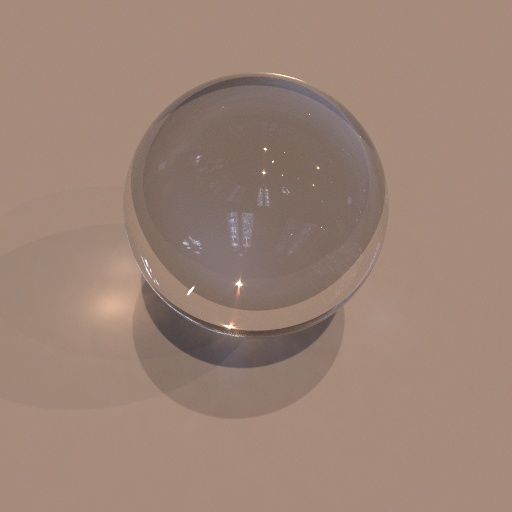
\includegraphics[width=0.45\linewidth]{figures/caustic-proj (1).jpg}}
    \hfill
  \subfloat[\label{1b}]{%
        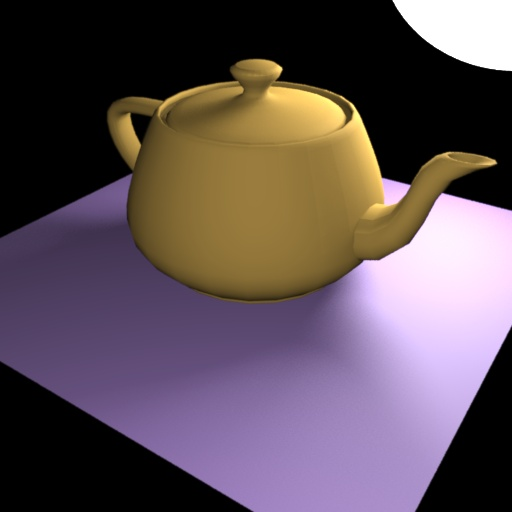
\includegraphics[width=0.45\linewidth]{figures/teapot-area-light.jpg}}
    \\
  \subfloat[\label{1c}]{%
        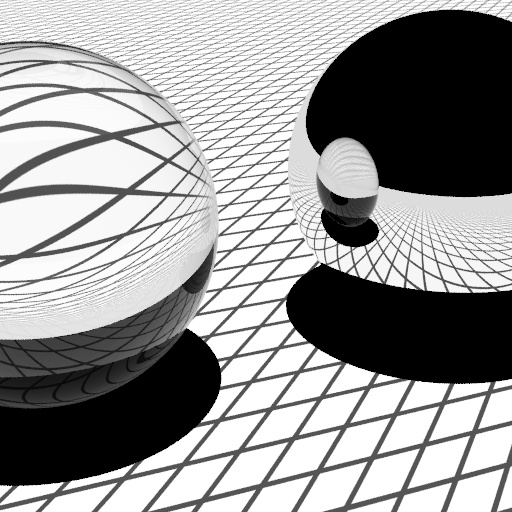
\includegraphics[width=0.45\linewidth]{figures/spheres-differentials-texfilt.jpg}}
    \hfill
  \subfloat[\label{1d}]{%
        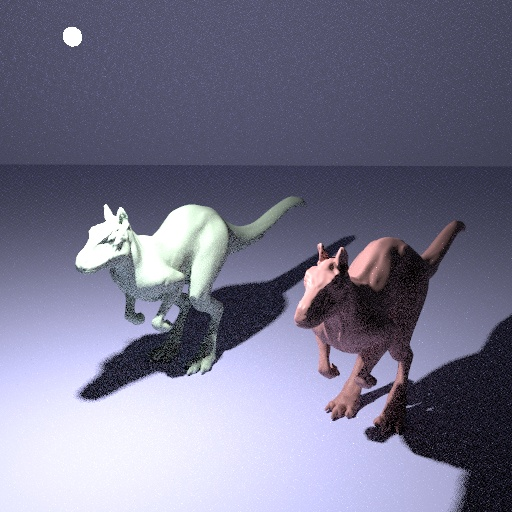
\includegraphics[width=0.45\linewidth]{figures/killeroo-simple.jpg}}
  \caption{Chosen Scenes used to validate performance with PBRT-V3. (a) scene 1 , caustic-proj \cite{PBRTdata}, (b) scene 2, teapot-area-light \cite{PBRTdata}, (c) scene 3, spheres-differentials-texfilt \cite{PBRTdata}, and (d) scene 4, killeroo-simple \cite{PBRT}.}
  \label{fig_scenes} 
\end{figure}



\subsection{Theoretical Background}
Image rendering is important in video industries like movies, animation, 3D video games, an so on because, rendering is the process of creating an image from a 3D scene description. PBR try to imitate reality by modeling the interplay of light and matter using real physics concepts \cite{PBR}. \par
The accelerator is one of the studied factors in this research, as was mentioned, two possibilities are analyzed, the kd-tree and BVH, kd-tree is a variation of Binary space partitioning (BSP) trees, which subdivide space with planes, however, kd-tree  restricts the divided plane to be perpendicular to one of the coordinate axes; which makes  creation of the tree more efficient. Meanwhile, BVH is a  ray intersection acceleration method based on primitive subdivision, which are partitioned into a hierarchy of separate sets  \cite{PBR}.\par
PBR involves vector and infinitesimal calculus of complex real-physics equations, therefore, it really takes advantage of the software and hardware resources to carry out the rendering, so it is a good option to evaluate the performance of the OS in their different scenarios.
\subsection{Related Work}
In \cite{duran2006analisis} analyzed web programming tools (PHP, ASP and JSP) using the Operative System Linux and Windows, they studied variables like Answer time, complexity, data base integrity and other. However, their focus is not the OS performance, and even so, 
\section{Conclusions}
The designed 


\bibliographystyle{IEEEtran}
\bibliography{bibliography.bib}
%https://www.quora.com/How-can-I-test-data-for-a-uniform-distribution
%http://rstudio-pubs-static.s3.amazonaws.com/433558_30d5068dd9fe45d58243c018c7582fc0.html
%https://stackoverflow.com/questions/44912747/plot-histogram-for-discrete-data

$256 \times 256$
\end{document}

